% !TeX spellcheck = zh_CN
% !BIB program = bibtex
\documentclass[aps,pre,12pt,preprint,%
	onecolumn,showpacs,showkeys,nofootinbib]{revtex4-1}
%UnlimitedFonts
	\def\hmmax{0}
	\def\bmmax{0}
%SVG
	\usepackage{svg}
%Tables
	\usepackage{array,booktabs,tabularx,multirow}
	\newcolumntype{C}[1]{>{\hsize=#1\hsize%
		\centering\arraybackslash}X}
%Math&Fonts
	\let\latexointop\ointop
	\usepackage{mathtools,amssymb,bm % basics
		,physics,siunitx,slashed % physics
		,esint,nicefrac,extarrows,mathrsfs % more symbols
		,calligra,romannum,dsfont,fourier-orns % nice fonts
		,eqnarray,resizegather,empheq % more envs
		,relsize,stackengine % utils
	}
%	\usepackage{amsthm}
	\usepackage[scr=esstix]{mathalfa}
	\usepackage[only,sslash]{stmaryrd}
	%DisplaySetup
	\newcommand*\bbox[1]{\fbox{\hspace{1em}\addstackgap[5pt]{#1}\hspace{1em}}}
	\empheqset{box=\bbox}
	\mathtoolsset{showonlyrefs}
%Utils
	%Legacy \oint
	\let\ointop\undefined
	\let\ointop\latexointop
	%Calligra
	\DeclareMathAlphabet{\mathcalligra}{T1}{calligra}{m}{n}
	\DeclareFontShape{T1}{calligra}{m}{n}{<->s*[2.2]callig15}{}
	%CosmeticTweaks
	\newcommand\inlineeqno{\stepcounter{equation}\ (\theequation)}
	\newcommand\scalemath[2]{\scalebox{#1}{\mbox{\ensuremath{\displaystyle #2}}}}
	\newcommand\raisemath[2]{\raisebox{#1\depth}{${#2}$}}
	\newfontfamily\signature{Vladimir Script}
	\newcommand{\newparagraph}{\pagebreak[3]
		\noindent\hfil%
		\raisebox{-4pt}[10pt][10pt]{\leafright~\qquad~\leafleft}%
		\par\nopagebreak%
	}
%CustomCmds
	%Brackets
	\DeclarePairedDelimiter\ave{\langle}{\rangle}
	\DeclarePairedDelimiterX\inprod[2]{\langle}{\rangle}{#1,#2}
	%Basics
	\newcommand{\mbb}[1]{\mathbb{#1}}
	\newcommand{\mrm}[1]{\mathrm{#1}}
	\newcommand{\mcal}[1]{\mathcal{#1}}
	\newcommand{\mscr}[1]{\mathscr{#1}}
	\newcommand{\tup}[1]{\textup{#1}}
	\newcommand{\mop}[1]{\operatorname{#1}}
	%Extras
	\newcommand{\scriptr}{\mathcalligra{r}\,}
	\newcommand{\rvector}{\pmb{\mathcalligra{r}}\,}
	\newcommand{\hodgedual}{\operatorname{\star}}
	\newcommand{\dual}{\ \xlongleftrightarrow{\ \textrm{dual}\ }\ }
	\newcommand{\idty}{\mathds{1}}
	\newcommand{\proj}[1]{\operatorname{%
		proj_{\mathit{#1}}}}
	\newcommand{\propsim}{\mathbin{\ensurestackMath{
		\stackunder[2pt]{\propto}{\sim}
	}}}
	\newcommand{\textbox}[1]{\fbox{#1}}
	\newcommand{\pdd}[1]{\operatorname{\partial_{\mathnormal{#1}}}}
	\newcommand{\cdd}{\operatorname{D}\!}
	\newcommand{\cdv}[1]{\operatorname{%
		\nabla_{\!\mathit{#1}\!}}}
	\newcommand{\ldv}[1]{\operatorname{%
		\mcal{L}_{\!\mathit{#1}\!}}}
	\newcommand{\ric}[1]{\operatorname{%
		Ric}\!\pqty{#1}}
%Hacks
	% physics.sty <texmf-dist/tex/latex/physics/>
	% USER: more spacing around Dirac's middle vert
	\newcommand{\xmiddle}[1]{\mspace{1mu}\middle#1\mspace{1mu}}
	\DeclareDocumentCommand\innerproduct{ s m g }
	{ % Inner product
		\IfBooleanTF{#1}
		{ % No resize
			\IfNoValueTF{#3}
			{\vphantom{#2}\left\langle\smash{#2}\xmiddle\vert\smash{#2}\right\rangle}
			{\vphantom{#2#3}\left\langle\smash{#2}\xmiddle\vert\smash{#3}\right\rangle}
		}
		{ % Auto resize
			\IfNoValueTF{#3}
			{\left\langle{#2}\xmiddle\vert{#2}\right\rangle}
			{\left\langle{#2}\xmiddle\vert{#3}\right\rangle}
		}
	}

%Miscellaneous
%	\newcommand{\tabindent}{\hspace{2em}}
	\newcommand{\naItl}{\tup{NaI\,(Tl)}}
	\newcommand{\perc}[1]{\SI{#1}{\percent}}
	\newcommand{\csAtom}{${}^{137}\mrm{Cs}$}
	\newcommand{\coAtom}{${}^{60}\mrm{Co}$}
\begin{document}
%Basic Data
	\title{%
	\texstringonly{\hfil\\[2\baselineskip]}
	\sf\LARGE%
		NaI\,(Tl)闪烁谱仪测定$\gamma$射线能谱%
	\texstringonly{\vspace{3ex}}}
	\author{\fangsong\large%
		Bryan%
	\vspace{2mm}}
	\affiliation{\it%
		北京大学物理学院~~学号:\normalfont 1500066666\,}
	\date{\today}
	\keywords{}
	\email{masked_email_please_contact@github.com}

\begin{abstract}
\vspace{10mm}
\begin{spacing}{1.5}\normalsize
\setlength{\parskip}{.3\baselineskip}
%	200—300字,
%	说明用什么方法做了什么事,
%	由此得到什么结果和结论,
%	有何意义.
%	不用缩略词,不用第一人称.
%%%%%%%%%%%%%%%%%%%%%%%%%%%%%%%%
	本实验利用\naItl 闪烁谱仪,探讨了$\gamma$射线与物质相互作用的基本规律,以及闪烁体探测器的基本工作原理。
	
	具体而言,实验中首先结合单道脉冲幅度分析器,利用\naItl 闪烁体探头采集了\csAtom 源的$\gamma$全能谱,随后结合\csAtom 源和\coAtom 源的峰位对谱仪进行了能量刻度;在此基础上,利用多道分析器再次获得了\csAtom 源的全能谱,并进一步测定了\csAtom, \coAtom 的混合能谱。
\end{spacing}
\end{abstract}

\maketitle
\thispagestyle{titlepagestyle}

%%  课程实验报告应假定读者既不是已知全部实验细节的指导教师,也不是缺少专业知识的公众,而是同领域的实验研究者,或审稿人. 不能要求读者要在读过课程讲义后才能读懂课程实验报告.
%%  凡不是自己独立思考得到的内容都应该引参考文献. 不能大段引用同一参考文献. 对复杂问题,应该优先考虑引用参考文献得到结果. 对简单一些的问题才鼓励独立思考.
\section{引言}
%%	研究论文引言一般包含以下内容:
%%	(1)所研究领域背景和现状;
%%	(2)有待研究的问题;
%%	(3)本研究的目的、主要内容和结果;
%%	(4)结果的意义.\par
%%	在写实验报告的引言时,同学可以假想自己是第一个做类似研究的人.\par
%%	引言一定要切合报告正文,不能漫无目的地介绍背景. 要快速地将读者引导到报告主题上,并作较深入的讨论.\par
%%	引言篇幅可以在较大范围内变化,但最长不应超过报告文字篇幅的1/3.\par
%%	引言撰写可以参考实验讲义,可以复述,但不能复制讲义上的任何一句话.\par
%%%%%%%%%%%%%%%%%%%%%%%%%%%%%%%
\vspace{-1ex}
	闪烁体探测器是利用某些物质在射线作用下会发光的特性对射线进行探测的仪器;射线通过闪烁体时,闪烁体的发光强度与射线在闪烁体内的能量损失有确定的关系,因此可以定量地探测射线的能量和强度。
	
	闪烁体及其上述特性很早就为人们所知;早在1903年,首创阴极射线管的Sir~W.~Crookes即发明了\tup{ZnS}闪烁镜(spinthariscope)以观察$\alpha$射线引起的闪光\supercite{crookes1903certain}。现代的闪烁体探测器诞生于曼哈顿计划,由Sir~S.~C.~Curran于1944年发明\supercite{curran1949counting};结合1930年代发明的光电倍增技术,现代的闪烁体探测器具有定量测量能力。
	
	由于射线与闪烁体之间存在多种相互作用,探测仪既可以可以探测带电粒子,又可以探测中性粒子,其探测效率高,分辨时间短。这些优秀的特性使得闪烁探测器在核物理研究和放射性同位素的测量中都得到了非常广泛的应用。
	
	在核物理实验中,\naItl 闪烁体探测器是最为常见的一类。本实验对\naItl 闪烁谱仪的结构进行了初步研究,通过\csAtom 源、\coAtom 源的能谱,对谱仪进行了能量刻度,鉴定了其的能量分辨率与线性,旨在认识$\gamma$射线与物质相互作用的规律,及闪烁谱仪的基本原理与特性。
\vspace{-.5\baselineskip}
\section{理论}
\vspace{-1ex}
%\setlength{\jot}{0pt}
	\naItl 闪烁谱仪的前端探头结构如图 \ref{fig:NaIdetector} 所示;首先,射线与闪烁体作用使之“闪烁”发光,产生光脉冲信号;闪烁体的放光强度反映射线在闪烁体内的能量损失,由此可以定量测得射线\textbf{能量}。闪烁光脉冲在光电倍增管的光阴极处经光电效应转化为光电子,电子经光电倍增后被阳极接收产生电压脉冲信号。
	
	另一方面,当闪烁体的发光衰减时间$\tau$充分短,小于射线与其相互作用的事件间隔时,可区分不同的相互作用事件并加以计数。对本实验采用的\naItl 而言,$\tau\sim\SI{1}{\us}$量级,具有充分高的时间分辨本领,计数电脉冲信号即可得放射线的\textbf{强度}。
\clearpage
	
	\begin{figure}[!ht]
		\centering
		\includesvg[width=.9\linewidth]{img/PhotoMultiplierTubeAndScintillator.svg}
		\hfil\vspace{1.5ex}
		\caption[闪烁体探头的工作原理示意图]{%
			闪烁体探头的工作原理示意图,选自 \cite{wiki:ScintillationCounter}. %
		}
		\label{fig:NaIdetector}
		\vspace{-1\baselineskip}
	\end{figure}
\subsection{$\gamma$射线与闪烁体的相互作用}
	实验中测定的是\csAtom 源、\coAtom 源的$\gamma$能谱,以此反映$\gamma$光子与物质——此时为\naItl 闪烁体——的相互作用。这包含:
	\begin{enumerate}[label=\arabic*.]
	\item \textbf{光电效应:}束缚电子完全吸收光子能量$E_\gamma$, 逸出成为光电子;电离能$E_i\ll E_\gamma$时,光电子动能$E = E_\gamma - E_i \simeq E_\gamma$. 对能谱的贡献为$E_\gamma$处的一尖峰。
	\item \textbf{Compton散射:}光子与电子发生弹性散射,能量部分转移;散射光子能量:
	\begin{equation}
		E_{\gamma'} = E_\gamma \bigg/ \pqty\Big{
			1 + \alpha\,(1 - \cos\theta)
		},\quad
		\alpha = \frac{E_\gamma}{m_e c^2}
	\end{equation}
	其中$m_e\simeq\SI{.511}{\MeV/c^2}$为电子质量,$\theta$为散射角。散射电子动能为$E = E_\gamma - E_{\gamma'}$, 随散射角$\theta\in\bqty{0,\pi}$递增,最大为:
	\begin{equation}
		E_{\max} = E_\gamma\,\frac{2\alpha}{1 + 2\alpha}
		\simeq \SI{.478}{\MeV},\quad
		\textit{若$E_\gamma = \SI{.662}{\MeV}$ \csAtom 源}
	\end{equation}
	\end{enumerate}
	
	Compton散射对能谱的贡献比较复杂,依赖其微分散射截面;基于量子电动力学导出的Klein–Nishina公式,可得Compton散射的微分散射截面如图 \ref{fig:ComptonSection} 所示。
\clearpage
	\begin{figure}[!ht]
		\centering
		\includegraphics[width=.5\linewidth]{img/Klein-Nishina_distribution.png}
		\caption[Compton散射的微分截面]{%
			\tup{Compton}散射的微分散射截面,选自 \cite{wiki:klein-nishina}. %
		}
		\label{fig:ComptonSection}
		\begin{explain}\footnotesize
			\hspace{2em}图中圆周上标记的坐标为散射角$\theta/\si{\deg}\in\bqty{0,180}$, 不同$E_\gamma$对应的微分截面相对大小以不同颜色的曲线标记。可见,当$E_\gamma\ll m_e c^2$时(图中蓝线)微分截面与经典的\tup{Thomson}散射一致,正比于$\frac{1 + \cos^2\theta}{2}$, 微分截面关于$\theta = \frac{\pi}{2}$对称,即向前、向后散射截面对称。增大$E_\gamma$, 散射截面减小,且向前、向后散射截面不再对称;向前散射的概率大于向后散射。
		\end{explain}
		\vspace{-1\baselineskip}
	\end{figure}
	
	具体而言,记$p = \frac{E_{\gamma'}}{E_\gamma} = \frac{1}{1 + \alpha\,(1 - \cos\theta)}$, Klein–Nishina公式给出\supercite{zee2010quantum}:
	\begin{equation}
		\dv{\sigma}{\Omega}
		\propto p^2 \pqty\big{p + p^{-1} - \sin^2\theta} \Big/ 2
	\end{equation}
	当$\alpha = \frac{E_\gamma}{m_e c^2}\to 0$时$p\to 1$, 上式回归经典Thomson散射$
		\dv{\sigma}{\Omega}
		\propto\frac{1 + \cos^2\theta}{2}
	$. 由于散射电子动能$E = E_\gamma - E_{\gamma'}$随散射角$\theta\in\bqty{0,\pi}$单调递增,直接可得截面关于$E$的分布:
	\begin{equation}
		\dv{\sigma}{E}
		= \dv{\sigma}{\theta} \bigg/ \dv{E}{\theta}
		= 2\pi\sin\theta\,\dv{\sigma}{\Omega} \bigg/ \dv{E}{\theta}
		\label{eq:comptonSectionByEnergy}
	\end{equation}
	
	代入$E = E_\gamma\pqty\big{
		1 - \frac{1}{1 + \alpha\,(1 - \cos\theta)}
	}$, 注意到在$E = 0, E_{\max}$处$\dv{E}{\theta} = 0$, 据 \eqref{eq:comptonSectionByEnergy} 可知这对应能谱上的峰值,而$0 < E < E_{\max}$则为一低于左右峰值的平台。
\clearpage
	
	具体计算可得Compton散射对能谱的贡献如下(代码参见附录):
	\begin{figure}[!ht]
		\vspace{-.5\baselineskip}
		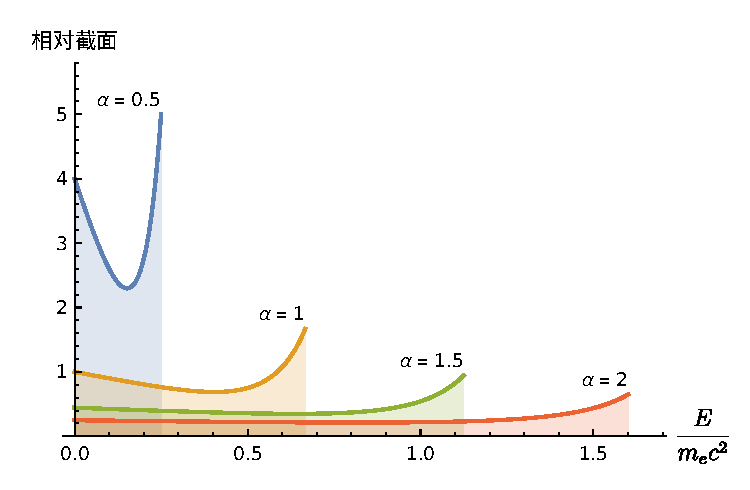
\includegraphics[width=.75\linewidth]{img/plots/comptonSpectrum.pdf}
		\caption[Compton散射对能谱的贡献]{%
			不同$\alpha = \frac{E_\gamma}{m_e c^2}$时
			\tup{Compton}散射对能谱的贡献
		}
		\label{fig:ComptonSpectrum}
		\vspace{-.5\baselineskip}
	\end{figure}
\FloatBarrier\noindent
	由于能量分辨率有限,实测结果将不具有上述尖锐峰值,而是存在一定的展宽;通过与正态分布卷积,模拟实测结果如下:
	\begin{figure}[!ht]
		\vspace{-.5\baselineskip}
		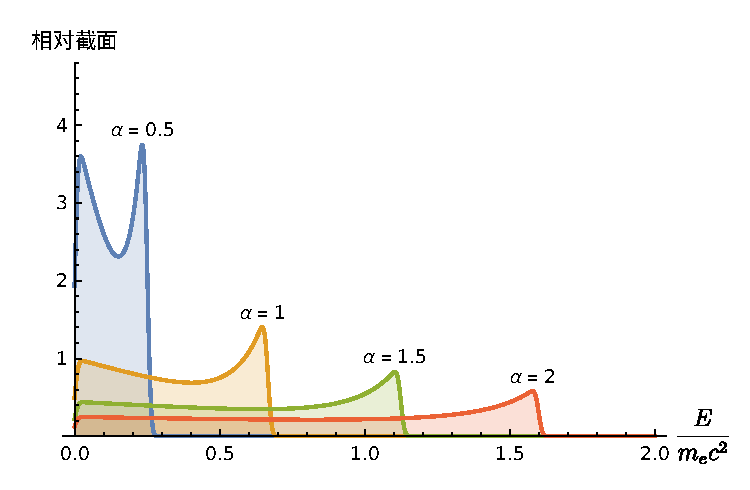
\includegraphics[width=.75\linewidth]{img/plots/comptonSpectrumObs.pdf}
		\caption[考虑仪器响应时的Compton能谱]{%
			考虑仪器响应时的\tup{Compton}能谱,通过与$\sigma = \num{.01}$的正态分布卷积得到。
		}
		\label{fig:ComptonSpectrumObs}
		\vspace{-.5\baselineskip}
	\end{figure}
\clearpage
	
	此外,Compton散射后的$E_{\gamma'}$可能进一步发生光电效应转化为光电子,据 \cite{textbook}, 由于这一过程十分迅速,无法在本实验仪器的时间分辨下加以区分,因此实际上$E_{\gamma'}$光电子和Compton电子$E$的信号将会叠加:$E_{\gamma'} + E = E_\gamma$, 即结果与光电峰重合,故称实测的$E_\gamma$峰为\textit{全能峰}。
	
	另外,入射$\gamma$光子可能穿过\naItl 晶体直接打到光电倍增管上发生 \ang{180} 反散射,产生的散射光子$E_{\gamma'} = E_\gamma - E_{\max}$进一步发生光电效应,将贡献反散射峰;对$E_\gamma = \SI{.662}{\MeV}$的\csAtom 源,有$E_{\gamma'} = \SI{.184}{\MeV}$. 
		
	\begin{enumerate}[start=3,label=\arabic*.]
	\item \textbf{正负电子对产生:}当$\gamma$光子能量超过$2m_e c^2 \simeq \SI{1.022}{\MeV}$之后,可受核或电子的库伦场作用转化为正负电子对;其对能谱的贡献为$m_e c^2 = \SI{.511}{\MeV}$处的特征谱线,由正负电子湮灭产生。
	\end{enumerate}
	
	注意到$\gamma$射线与物质的直接作用产物多为电子;在闪烁体中,这些电子的动能转化为特定波长范围内的闪烁光子。对\naItl 而言,其闪烁光谱主要为 \SI{415}{\nm} 附近的蓝光\supercite{sodium-iodide:online}。
	
	对\csAtom 源$E_\gamma = \SI{.662}{\MeV} < 2m_e c^2$, 不足以产生正负电子对,其能谱中的特征峰位即全能峰 \SI{.662}{\MeV} 与反散射峰 \SI{.184}{\MeV}. 对\coAtom 源,本身即放出两种能量(\SI{1.17}{\MeV}, \SI{1.33}{\MeV})的射线,因此我们主要关注相应的两个全能峰。
%\restorejot
%%%%%%%%%%%%%%%%%%%%%
\section{实验装置}
\vspace{0\baselineskip}
%%	在此部分需要将实验条件交待清楚到别人能重复你的实验结果的程度. 此外,还需表明你已尽了最大努力来提高实验精度和结果的可靠性. 简单的不确定度估计可以在此节给出,复杂一些的可以放到分析讨论部分.\par
%%	实验条件不仅是指直接影响实验结果的实验参量,而且还包括影响实验质量和可靠性的因素,如室温、空气湿度、基真空、原材料纯度等.\par
%%	作为教学实验报告,此节写详细一点没有坏处.\par
%%	成段有叙述,必要才分节。
%%%%%%%%%%%%%%%%%%%%%%%%%%%%%%%
	\naItl 闪烁谱仪由前述闪烁体探头(含光电倍增管)及后端仪器组成。探头后端,电压信号经进一步线性放大后,可由示波器显示脉冲波形,亦可输入单道分析器进行脉冲幅度分析,或输入微机多道自动化地获得入射射线的能谱。
	
	其中,单道分析器只容许$V\to V + \Delta V$幅度的脉冲通过,$V$为阈值,而$\dd{V}$对应道宽;微机多道原理类似,只不过可以同时对一定范围内的所有脉冲间隔$V_x\to V_{x+1} = V_x + \Delta V$进行监测计数,$x$即道址,由此可极大提高效率。
\clearpage
\section{结果与分析}
%	实验结果应尽量以图表的形式给出. 每一个图表都应该是完整的,即阅读图表时可以不必依赖正文.\par
%	依自己意愿,实验结果和对结果的分析讨论既可分为两节也可合在一节.\par
%
%	每个图一般包含:图名、轴名、轴、刻度、标尺、数据点、曲线、图例、标注和图注等部分. 应尽量让读者不看正文就能基本理解图的含意.\par
%	逐点测量得到的函数关系要同时用表格和图给出. 需要作比较的多条曲线要画在同一图上.\par
%	为避免读者在图表和正文间反复跳跃阅读,在正文中也要对图表作必要的说明.\par
%
%	对于预料之外的实验结果,必须首先小心证明其可靠性.读者只有在相信你的实验结果时才愿意花时间看你的分析.\par
%	必须用文字归纳整理出正式的实验结果或结论.可信的实验结果是课程报告最重要的内容.作为一个实验物理工作者,分析解释出错并不丢脸,实验结果不被采信则是致命的.\par
%	教学实验的结论往往是预先知道的. 所以,教师更关心的是你的说理过程. 一般说来,单由课内实验的结果不足以能得到明确的结论. 此时,你可以引用他人的研究结果来帮助帮助自己的论证,但必须注明出处. \par
%	确实不能得到明确结论时,可以给出几种可能结论并指出可以再做哪些实验来帮助作进一步的判断.\par
%	总之,分析讨论部分要做到: 论据要valid,论证要reasonable,结论要convincing.\par
%%%%%%%%%%%%%%%%%%%%%%%%%%%%%%
\vspace{0ex}
	
	首先利用单道逐点计数测定 \csAtom 全能谱,固定道宽 \SI{.1}{\V}, 结果如下:
	\begin{figure}[!ht]
	\centering
	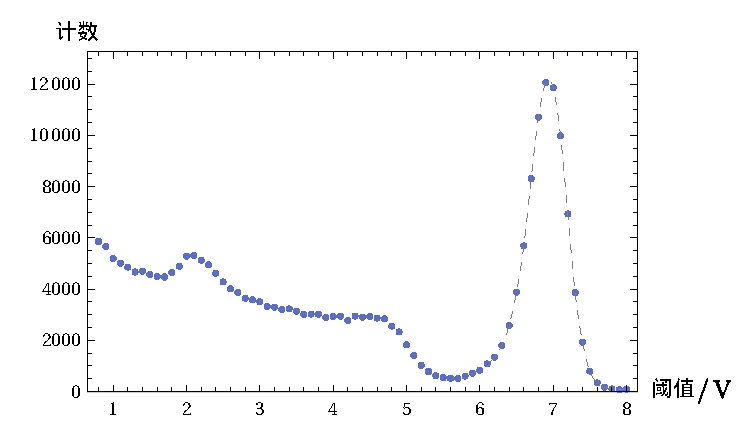
\includegraphics[width=.85\linewidth]{img/plots/spectrumPlot.pdf}
	\caption{\csAtom 源全能谱,由\naItl 闪烁谱仪结合单道计数测得}
	\vspace{-1ex}
	\end{figure}
\FloatBarrier\noindent%
	可见最强的全能峰,以及图中单道阈值 \SI{2}{\V} 附近的反散射峰。Compton平台及其边沿与理论预测大致吻合。
	
	在此基础上,利用前述\csAtom 源和\coAtom 源的特征峰值对谱仪进行能量刻度;将线性放大倍数减小一半以涵盖\coAtom 源的较高能峰位,相应地预计\csAtom 源峰位对应的阈值大致为上图显示的一半左右。在预估的峰值附近取点,测得对应峰位如下:
	\begin{table}[!ht]
	\caption{实测特征峰值对应的单道阈值}\small
	\begin{tabularx}{.5\linewidth}{C{1}C{1}}
	\toprule\midrule
		能量 / $\si{\MeV}$ & 单道阈值 / $\si{\V}$ \\
	\midrule
		0.184 & 1.05 \\
		0.662 & 3.56 \\
		1.17  & 5.95 \\
		1.33  & 6.78 \\
	\midrule\bottomrule
	\end{tabularx}
	\end{table}
\clearpage
	
	线性拟合,可得阈值与能量的关系如下:
	\begin{figure}[!ht]
	\centering
	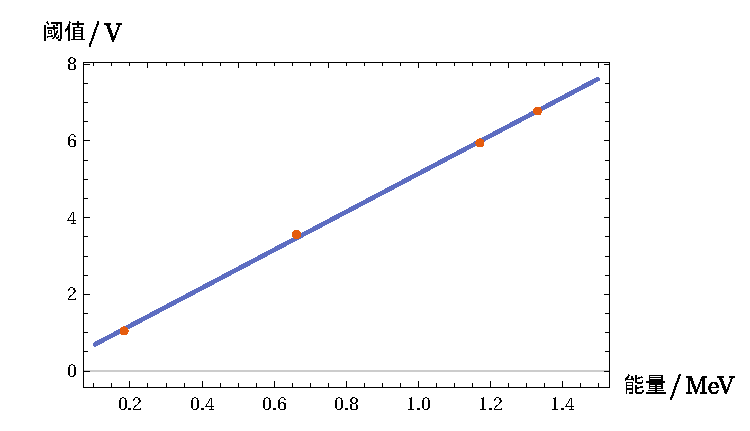
\includegraphics[width=.8\linewidth]{img/plots/linearModel.pdf}
	\caption{实验用\naItl 谱仪的能量刻度}
%	\vspace{-1ex}
	\end{figure}
	\vspace{-.6\baselineskip}
	\begin{equation}
		X/\si{\V} \simeq 0.184 + 4.96\,\pqty{\frac{E}{\si{\MeV}}}
	\end{equation}
	其中$X$为单道阈值;可见谱仪给出良好的能量线性关系。进一步求反函数,即给出$E$对$X$的依赖:
	\begin{equation}
		\frac{E}{\si{\MeV}} \simeq -0.0372 + 0.202\,X/\si{\V}
	\end{equation}
	
	另外,利用\csAtom 谱的全能峰可估计谱仪的能量分辨率;插值寻峰得全能峰位:
	\begin{equation}
		X_0/\si{\V} \simeq 6.93763,\quad N \simeq 12175.5
	\end{equation}
	其中$N$为计数;考虑$\frac{N}{2}$给出的半宽$\Delta X_{1/2}$, 有:
	\begin{equation}
		\Delta X_{1/2}/\si{\V} \simeq 7.22613 - 6.61629
		\simeq 0.609839
		\quad\Longrightarrow\quad
		\epsilon = \frac{\Delta X_{1/2}}{X_0} \simeq\num{.088}
	\end{equation}
	
	最后,利用微机多道采集\csAtom 源、\coAtom 源的混合谱,并再次采集\csAtom 谱,采集定时均取为5分钟,结果如下:
	\begin{figure}[!ht]
	\vspace{-.3\baselineskip}
	\centering\small
	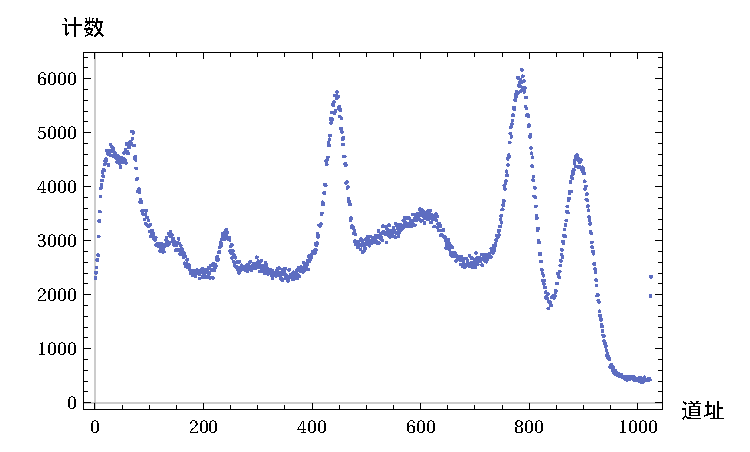
\includegraphics[width=.78\linewidth]{img/plots/mixedSpectrum.pdf}\\[1ex]
	(a) \textit{\coAtom、\csAtom 混合谱}\\[2ex]
	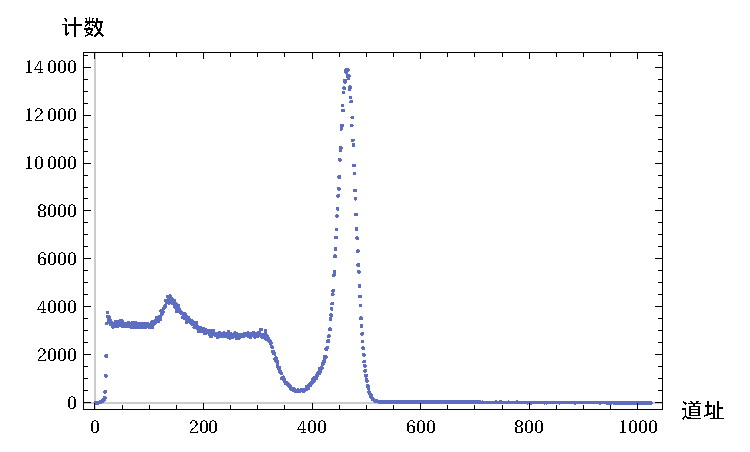
\includegraphics[width=.78\linewidth]{img/plots/csSpectrum.pdf}\\[1ex]
	(b) \textit{\csAtom 能谱}\\[1ex]
	\caption{实验所得微机多道能谱}
	\vspace{-.2\baselineskip}
	\end{figure}
\FloatBarrier\noindent
	特征峰位明显,与预期基本吻合。
	
\clearpage
%	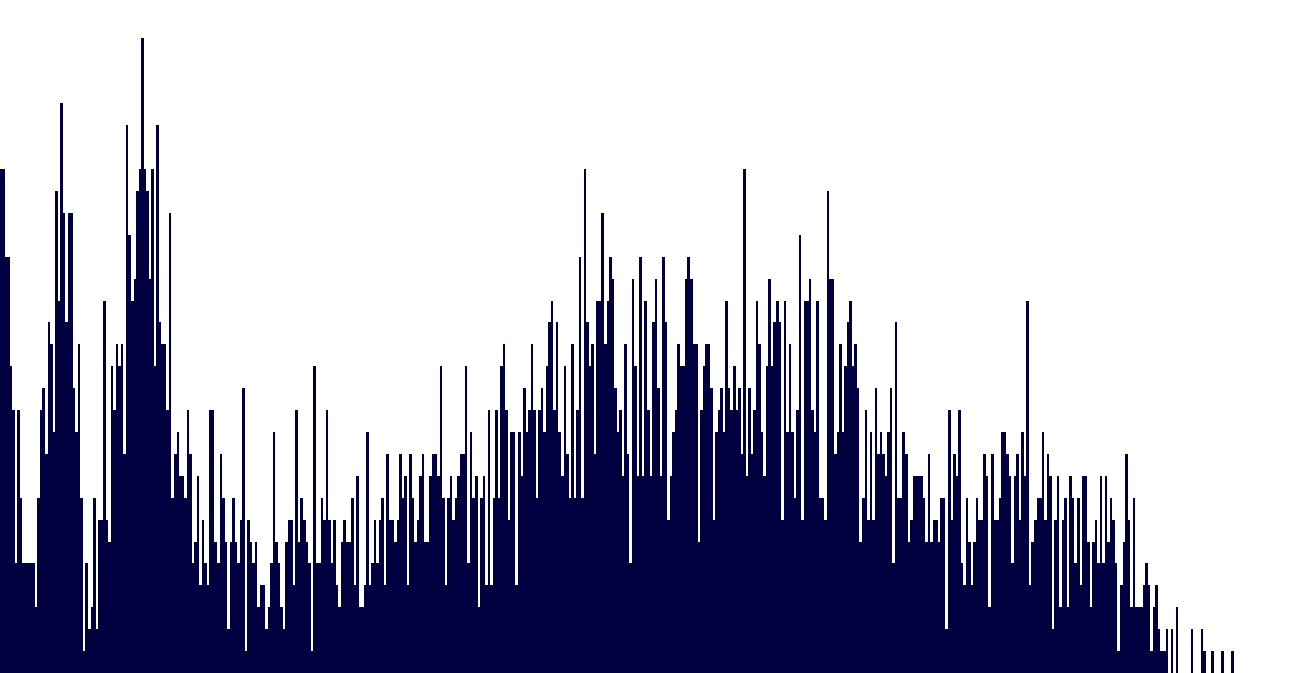
\includegraphics[
%		height=8\baselineskip,
%		width=.8\linewidth,
%		frame
%	]{data/bg_white.png}
%	\begin{table}[!h]
%	\vspace{0\baselineskip}
%	\caption[峰值道址]{参考穆斯堡尔谱的峰值道址}
%	\footnotesize
%	\textit{\tup{(1)} \FeAlpha}\\[1ex]
%	\begin{tabularx}{.85\linewidth}{%
%		C{1} | *6{C{.5}}
%	}
%	\toprule\midrule
%		序号 &
%			1 & 2 & 3 & 4 & 5 & 6 \\
%	\midrule
%		右侧峰道址$v_R$ &
%			289 & 327 & 367 & 396 & 436 & 475 \\
%		左侧峰道址$v_L$ &
%			226 & 186 & 147 & 117 & 77 & 38 \\
%	\midrule\bottomrule
%	\end{tabularx}
%	\label{tab:}
%	\vspace{-.3\baselineskip}
%	\end{table}%
\section{结论}
%%%	首先要给出实验结果,然后再给出由实验结果分析得到的结果和结论。此部分给出的内容要比摘要中的全面,用词要更准确。\par
%%%%%%%%%%%%%%%%%%%%%%%%%%%%%%%	
	实验结合单道脉冲幅度分析器,利用\naItl 闪烁体探头采集了\csAtom 源的$\gamma$全能谱,随后结合\csAtom 源和\coAtom 源的峰位对谱仪进行了能量刻度,并估计了谱仪的能量分辨率;在此基础上,利用多道分析器再次获得了\csAtom 源的全能谱,并测定了\csAtom, \coAtom 的混合能谱;以此探讨了$\gamma$射线与物质相互作用的基本规律,以及闪烁体探测器的基本工作原理。
\vspace{-.5\baselineskip}
\section{致谢}
%	此部分感谢同组人...和对实验和报告有帮助的人。
%%%%%%%%%%%%%%%%%%%%%%%%%%%%%%
	感谢付恩刚老师的细致指导和耐心帮助;感谢 \TeX\, - \LaTeX\, Stack Exchange\footnote{%
		\url{https://tex.stackexchange.com/}
	}, 助我解决了众多排版问题。

\vspace{.8\baselineskip}

\setlength{\bibsep}{1ex}
\linespread{1.}\selectfont
\bibliographystyle{../BibStyle/gbt-7714-2015-numerical}
%\bibliographystyle{apsrev4-1}
\bibliography{../BibStyle/Textbook,bib/Ref}
\clearpage


\linespread{1.5}\selectfont
\appendix
\section{Compton能谱的计算}
	利用Mathematica的符号与数值计算功能可以方便地推导、绘制Compton能谱的基本形态,代码如下:
	\begin{enumerate}
	\item \textbf{计算并绘制Compton截面的角分布:}\par\vspace{1ex}
	\qquad\qquad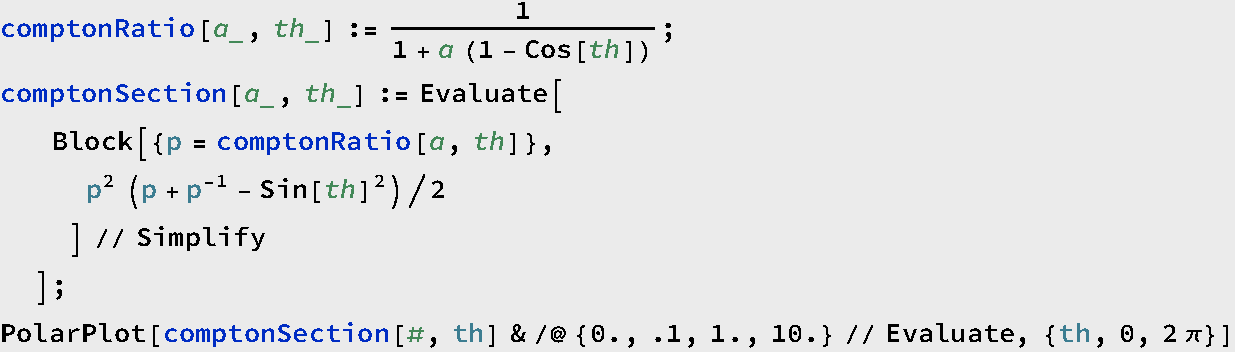
\includegraphics[scale=.6]{data/comptonAngleDist.pdf}
	\item \textbf{计算Compton能谱:}\par\vspace{1ex}
	\qquad\qquad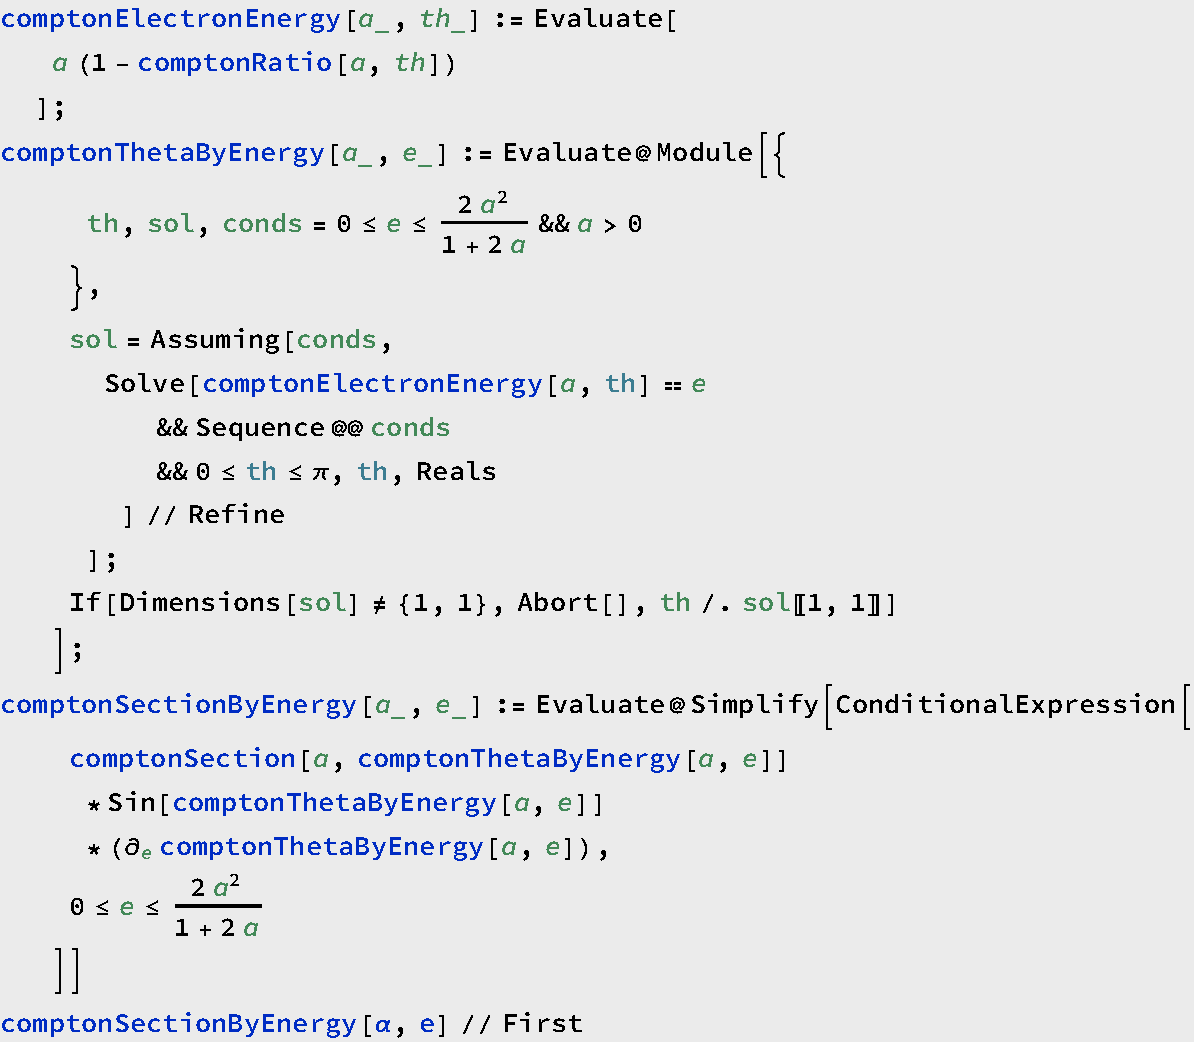
\includegraphics[scale=.6]{data/comptonSectionByEnergy.pdf}\par
	\qquad\qquad \textit{结果:}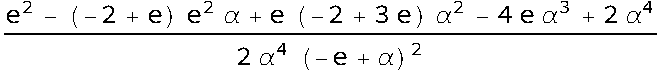
\includegraphics[scale=.6]{data/comptonSectionByEnergyOut.pdf}
	\item \textbf{绘制Compton能谱:}\par\vspace{1ex}
	\qquad\qquad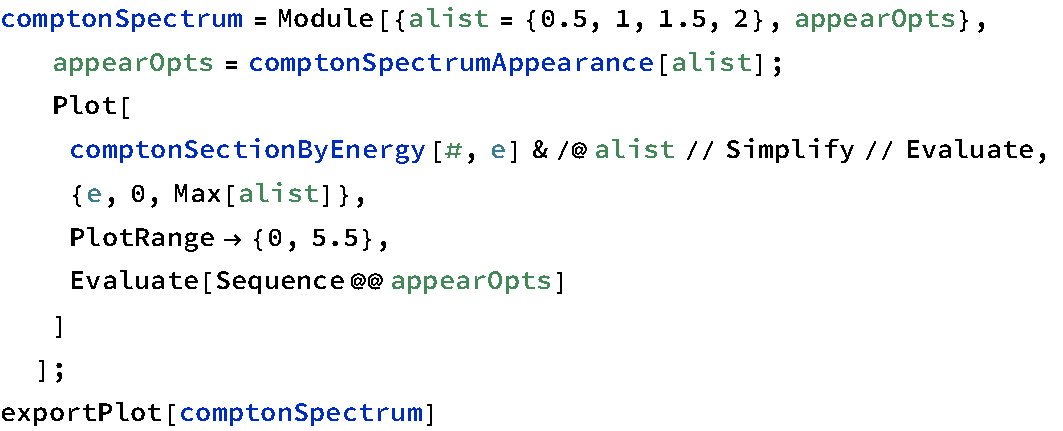
\includegraphics[scale=.6]{data/comptonSpectrumCode.pdf}
	\item \textbf{考虑仪器响应的Compton能谱:}\par\vspace{1ex}
	\qquad\qquad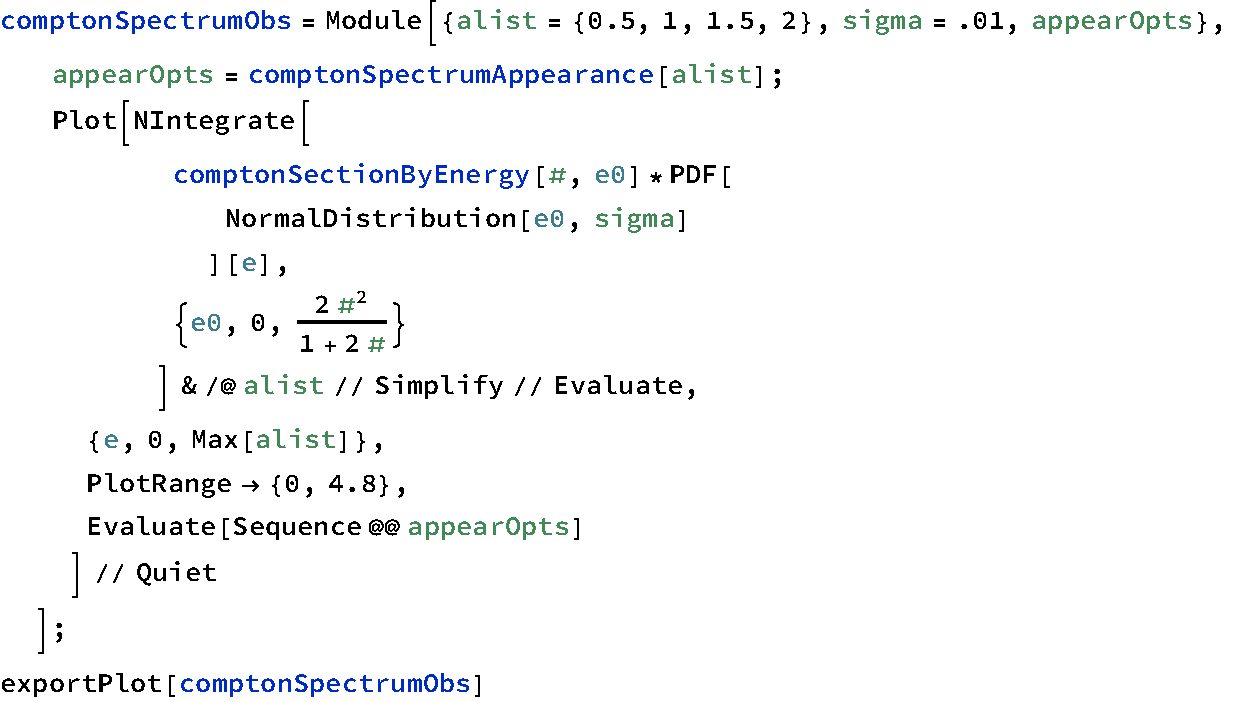
\includegraphics[scale=.6]{data/comptonSpectrumObsCode.pdf}
	\end{enumerate}
\clearpage
\end{document}